% ===========================================================================
%  Plotting your data using PGF/TikZ
% ===========================================================================
%  This chapter demonstrates the PGFPlots integration provided by AuroraTeX.
%  It shows both 2D and 3D plots, code snippets, and a description list
%  explaining common axis parameters.
% ===========================================================================

\Chapter{Plotting your data using PGF/TikZ}

\section{Introduction}

PGFPlots and TikZ are useful when the figure should stay editable inside the
source document. The template defines a small \inlinecode{aurora} axis style so
common plots share grid, label, and legend conventions.

% ------------------------------
%  excerpt box
% ------------------------------
\begin{excerpt}
PGF/TikZ describes vector graphics with TeX macros. That makes technical
figures portable, reproducible, and easy to keep visually consistent with the
rest of the report.
\end{excerpt}

\subsection{A Simple 2D Plot}

The following plot compares two functions and is computed by PGFPlots during
compilation.

% ------------------------------
%  2D PGFPlots figure — uses the `aurora` axis style
% ------------------------------
\begin{figure}[H]
  \centering
  \begin{tikzpicture}
    \begin{axis}[
      aurora,
      xlabel={$x$},
      ylabel={$f(x)$},
      domain=-10:10,
      samples=120,
      legend pos=north west
    ]
      \addplot[red, very thick] {x^3 - 7*x - 1};
      \addlegendentry{$x^3 - 7x - 1$}
      \addplot[blue, very thick] {x^2 + 2*x + 1};
      \addlegendentry{$x^2 + 2x + 1$}
    \end{axis}
  \end{tikzpicture}
  \caption{A 2D PGFPlots figure comparing two functions.}
  \label{fig:two-dimensional-plot}
\end{figure}

% ------------------------------
%  code block (LaTeX for the 2D plot)
% ------------------------------
\begin{lstlisting}[language={[LaTeX]TeX},style=AuroraListing]
\begin{axis}[aurora, xlabel={$x$}, ylabel={$f(x)$}]
  \addplot[red, very thick] {x^3 - 7*x - 1};
  \addlegendentry{$x^3 - 7x - 1$}
  \addplot[blue, very thick] {x^2 + 2*x + 1};
  \addlegendentry{$x^2 + 2x + 1$}
\end{axis}
\end{lstlisting}

% ------------------------------
%  description list — axis parameters explained
% ------------------------------
\begin{description}
  \item[domain] The range over which the function is calculated.
  \item[samples] The number of evaluations used to draw the curve.
\end{description}

\subsection{Plotting 3D plots}

Three-dimensional surfaces are also possible with the same axis system. The
example below uses a small sample count so compilation remains fast for a
template repository.

% ------------------------------
%  3D PGFPlots figure — surface plot with colormap
% ------------------------------
\begin{figure}[H]
  \centering
  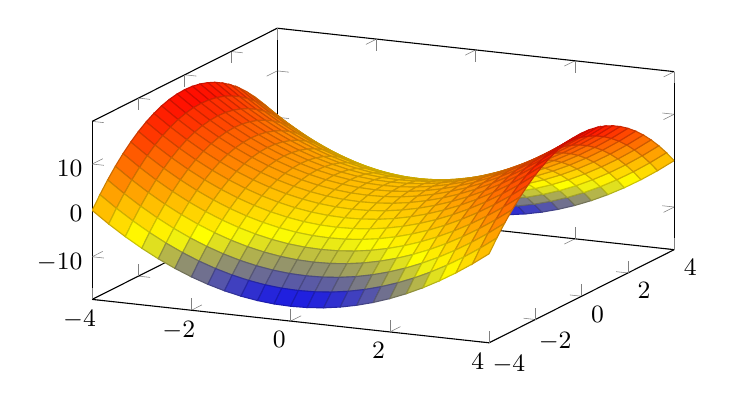
\begin{tikzpicture}
    \begin{axis}[
      view={25}{30},
      width=0.74\textwidth,
      height=0.46\textwidth,
      axis lines=box,
      colormap/hot,
      tick label style={font=\small},
      label style={font=\small}
    ]
      \addplot3[
        surf,
        shader=faceted,
        samples=25,
        domain=-4:4,
        y domain=-4:4
      ] {x^2 - y^2};
    \end{axis}
  \end{tikzpicture}
  \caption{An example 3D plot produced with PGFPlots.}
  \label{fig:three-dimensional-plot}
\end{figure}

% ------------------------------
%  code block (LaTeX for the 3D plot)
% ------------------------------
\begin{lstlisting}[language={[LaTeX]TeX},style=AuroraListing]
\begin{axis}[view={25}{30}, colormap/hot]
  \addplot3[
    surf,
    shader=faceted,
    samples=25,
    domain=-4:4,
    y domain=-4:4
  ] {x^2 - y^2};
\end{axis}
\end{lstlisting}

Because the figures are written as source, color, labels, legends, and data
ranges can be adjusted without replacing external image files.
